%----------------------------------------------------------------------------------------
%	PACKAGES AND OTHER DOCUMENT CONFIGURATIONS
%----------------------------------------------------------------------------------------

\documentclass[twoside,twocolumn]{article}


\usepackage[sc]{mathpazo}
\usepackage[T1]{fontenc} 
\linespread{1.05} 
\usepackage{microtype} 

\usepackage[english]{babel} 

\usepackage[hmarginratio=1:1,top=32mm,columnsep=20pt]{geometry} 
\usepackage[hang, small,labelfont=bf,up,textfont=it,up]{caption} 
\usepackage{booktabs} 
\usepackage{lettrine}
\usepackage{graphicx}

\usepackage{enumitem} 
\setlist[itemize]{noitemsep} 

\usepackage{abstract} 
\renewcommand{\abstractnamefont}{\normalfont\bfseries}
\renewcommand{\abstracttextfont}{\normalfont\small\itshape} 

\usepackage{titlesec} 
\renewcommand\thesection{\Roman{section}} 
\renewcommand\thesubsection{\roman{subsection}} 
\titleformat{\section}[block]{\large\scshape\centering}{\thesection.}{1em}{} 
\titleformat{\subsection}[block]{\large}{\thesubsection.}{1em}{} 

\usepackage{fancyhdr}
\pagestyle{fancy} 
\fancyhead{} 
\fancyfoot{} 
%\fancyhead[C]{ title $\bullet$ date} % Custom header text
%\fancyfoot[RO,LE]{\thepage} % Custom footer text

\usepackage{titling} 

\usepackage{hyperref} 
%----------------------------------------------------------------------------------------
%	TITLE SECTION
%----------------------------------------------------------------------------------------

\setlength{\droptitle}{-4\baselineskip} % Move the title up

\pretitle{\begin{center}\Huge\bfseries} 
\posttitle{\end{center}} 
\title{Problems that arise when peforming a small-scale soil microbiome analysis and how to prevent them} 
\author{
\textsc{Ilya Senatorov} \\
\normalsize University College London \\
}
\date{May 8, 2018}
\renewcommand{\maketitlehookd}{
\begin{abstract}
\noindent 
%
%ABSTRACT
%
%

\end{abstract}
}
\bibliographystyle{vancouver}
%----------------------------------------------------------------------------------------

\begin{document}

\maketitle

%	ARTICLE CONTENTS


\section{Introduction}

\lettrine[nindent=0em,lines=3]{M}icrobiome analysis is an area of research that relies heavily on large samples and big amounts of data \cite{Thompson2017}. In this research I describe our attempt to conduct a small-scale soil microbiome analysis and the problems that occurred.\\
One of the main areas of development in the field of microbiome analysis is the EMP - Earth Microbiome Project\cite{Gilbert2014}. It focuses on creation of a global catalogue of Earth's microbial diversity.


One of the main aims of the analysis was to check whether the samples we collected follow the general trends of diversity and to confirm that the sample can be added to the EMP database.

%-----------------------------------------------

\section{Methods}

The analysis was performed on 30 samples of soil, collected in Central London in October 2017. Metadata, such as moisture, temperature, footfall was collected on the spot, while other aspects, such as pH and concentrations of various ions was measured in the laboratory. Then 4 different kits were used in a workflow designed to extract the 16S V4 DNA region from the prokaryotes in the soil, following the instructions provided by manufacturer of each kit. \\
%
First, DNA was extracted using the \textit{DNeasy PowerSoil Kit}, and PCR primers were designed that contained Golay barcodes, allowing multiple samples to be sequenced simultaneously. \textit{BioMic PCR kit} was used with the aforementioned primers to perform the PCR. The mix acquired as the result of PCR was purified using \textit{QIAquick PCR Purification Kit}, and then the concentration of dsDNA was measured using \textit{SpectraMax Quant™ AccuClear Nano dsDNA Assay Kit}. Then all the samples were diluted to contain equal concentrations of DNA, and sequncing was performed on \textit{Illumina's MiSeq} sequncer. This workflow returned the raw DNA sequences that were used for downstream analysis.\\
%
Analysis of sequences was performed using the QIIME\footnote{Version 1.9.1} package\cite{Caporaso2010,Kuczynski2012}, which allows users to perform high-throughput sequence analysis. The basic pipeline consists of:
\begin{enumerate}
	\item Data validation - checks the input data for errors
	\item Sequence demultiplexing - recognises the Golay barcodes and splits data back into 30 samples.
	\item OTU picking - for sequence analysis, it is preferable to work not with sequences directly, but with OTUs - Operational Taxonomic Units, which in out case correlate with a single species.
\end{enumerate}
%
This pipeline sets the foundation for any further analysis and is generally the most expensive part of the analysis, in terms of computational power. It requires a referencing database, for which I used SILVA\cite{Quast2012}\footnote{Release 132, April 10, 2018}, which is more up-to-date than Greengenes\cite{McDonald2012}.\\



%------------------------------------------------

\section{Results}

During the OTU picking stage, I managed to recover over 4.5 million sequences overall, with 16448 of them being unique. However, it should be noted, that due to use of closed-reference OTU picking, which was used due to being cheaper, almost 800 thousand sequences (\~17\%) were removed from the analysis since no match was found in the database. This correlates with the  Because these sequences were not found in the database, it can be assumed that they were rare and could have severely influenced diversity of the samples.\\
%
Another issue that I can point out with the OTU picking method, is the limitation imposed by the databases. SILVA database currently contains 177222 sequences, which means that our study, while being rather small, already covered almost 10\% of the database. Thompson et al.\cite{Thompson2017} report that a study they performed using just under 100 samples from different biomes covered up OTU picking strategy is outdated, and with increase of computational power and decrease in price of core-hours of High Performance Computer clusters, other techniques (for example Deblur\cite{Amir}) will provide more accurate results. \\

\begin{figure}
	\includegraphics[width=\linewidth]{silva_greengenes_emp.jpg}
	\caption{Comparison of Greengenes with SILVA databases, with number of reads in EMP samples, grouped by environment. Boxplots show median, IQR, and 1.5 × IQR (with outliers). Adapted from \cite{Thompson2017}}
	\label{fig:EMP_Silva}
\end{figure}

In order to analyse our samples, I used the QIIME scripts, such as core\_diversity\_analyses.py, which allows users to take a look at basic properties of the microbial communities, such as alpha and beta diversities. However, it should be noted that while providing good results in terms of data, these workflows lack in the area of visualising data, which lead me to creation of my own visualisation scripts\cite{Senatorov2018}. They allow us to validate the results of our analysis , by using the data from the EMP, and points out the issues in the collected data.

\begin{figure}
	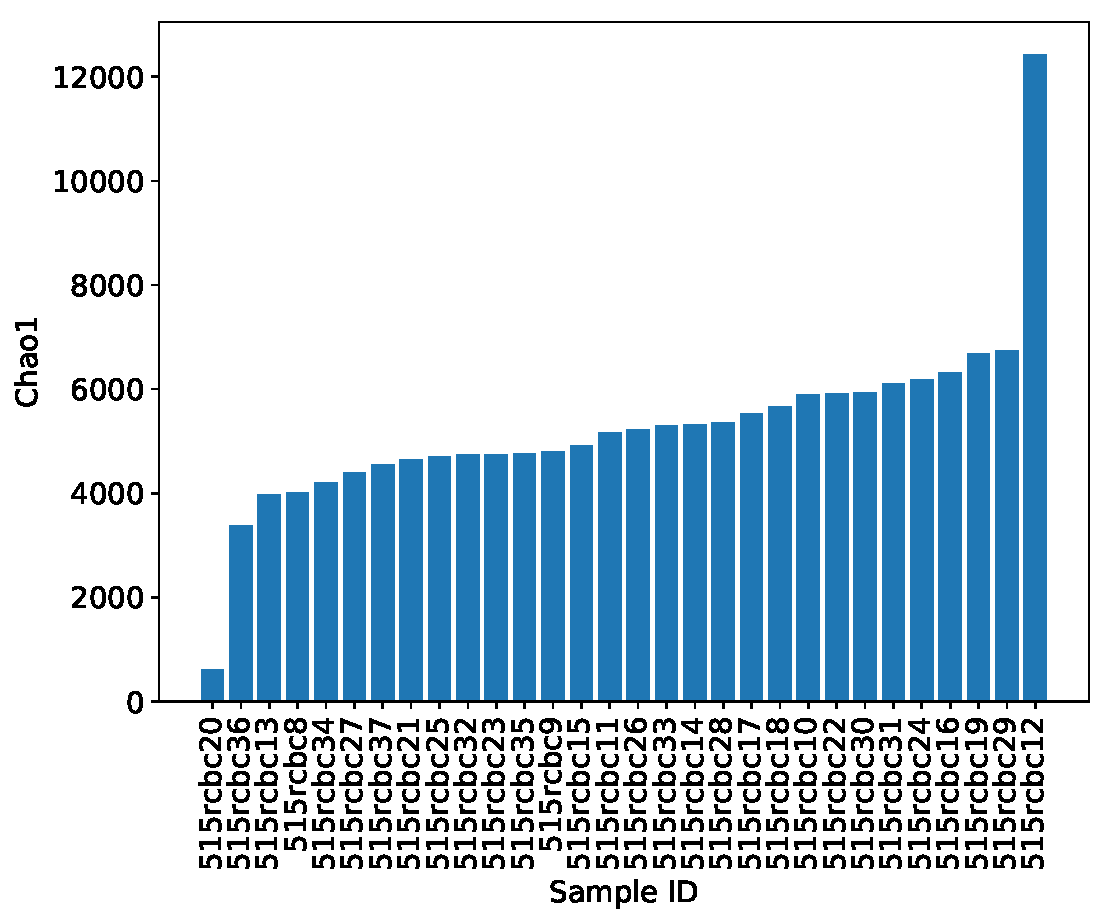
\includegraphics[width=\linewidth]{../analyses/figs/chao1_alpha.pdf}
	\caption{Alpha diversity (Chao1) for each of 30 samples. Obvious outliers can be seen.}
	\label{fig:alpha_diversity}
\end{figure}
%------------------------------------------------

\section{Discussion}


\newpage
%----------------------------------------------------------------------------------------
%	REFERENCE LIST
%----------------------------------------------------------------------------------------

\bibliographystyle{vancouver}
\bibliography{/home/ilya/Documents/Citations/3301.bib}

%----------------------------------------------------------------------------------------

\end{document}
